\appendix
\chapter{Theorems and Proofs}
\label{chap:append}
\lhead{Chapter \ref{chap:append}. \emph{\nameref{chap:append}}} %

%\section{Machine Specifications}
%\label{ann:specs}
%\begin{table}[H]
%	\begin{center}
%		\begin{tabular}{|c|c|}
%			\hline
%			Operating System  & Arch Linux 3.14.4 x64\\\hline
%			CPU & Intel i7 Dual-Core, 2GHz\\\hline
%			Memory & 8 GB, 1600 MHz \\\hline
%			Storage &  Solid-State Drive, 300 MB/s (read)\\\hline
%		\end{tabular}
%		\caption{Machine specifications}
%	\end{center}
%\end{table}

\section{Median of Medians}
\label{ann:median}
Efficiently constructing a balance \kdtree depends on an efficient method to pick the point that divides the hyper-rectangle in two. One way to reasonably quickly find a value close to the median is to find the median of a sample. To ensure the quality of this sample, is to gather the medians of smaller subsets which can be quickly calculated. This algorithm is an example of a \emph{selection algorithm} \cite{selection} and is known as the \emph{median of medians} algorithm \cite{medians}.

The median of medians algorithms works as follows. Any starting array $S$ consisting of $n$ arbitrary values is split into $n/5$ sub-arrays, each containing at most 5 elements (the last array might have less, depending on whether $n$ is divisible by 5 or not). For each of the sub-arrays, the median can be calculated in constant time, since for 5 values it can be done in at most 6 comparisons, which for the whole array $S$ takes $6n/5$ comparisons. After finding all the sub-arrays' medians and gathering them in a new array $F$, the algorithm then is called recursively for $F$ until only one value $M$ remains. $M$ is then used to partition the input into two sub-groups: elements smaller than $M$ and elements larger than $M$. The two subgroups are then concatenated in increasing order and with $M$ in between them, and the algorithm is recursively called again for the group that contains the $n/2$th point of the newly concatenated list. Whenever the list has less than a given number of elements, the median is calculated via brute-force, to avoid infinite recursion. This value will be the value returned by the initial recursive call of the function.

As stated above, this algorithm only returns a value close to the real median. Despite this, it can proven that for any array $S$, the value $M$ will always be between the 30th and the 70th percentiles. At each recursive stage, the values in $F$ larger than $M$ are discarded. This means that out of the $n/5$ values for any given vector, $n/10$ will be larger by definition, since $M$ is picked as the median. For each value in $F$ larger than $M$, there will also be two other values that are larger than $M$, since each value in $F$ was chosen as a median out of 5 different values. This means that the number of values greater than $M$ will be at most $3n/10$. Similarly, by a symmetric proof, there will also be $3n/10$ values in $S$ smaller than $M$. This also means that the second recursive call will at worst have $7n/10$ elements, which is a constant fraction of the input. This property is essential in proving the linear complexity of the algorithm.

Analyzing the time complexity $T()$ of this algorithm requires analyzing separatly both recursive calls of the algorithm. The first recursive call occurs in a list of size $n/5$, and takes $T(n/5)$ time. The second recursive call occurs in a list with $7n/10$ elements, which takes $T(7/n)$. Finding the median for a group of 5 elements requires a constant number of comparisons. These comparisons can be arranged in such way that only 6 are necessary for a group of 5 elements. This means that the algorithm has a constant factor of $6/5$ for calculating a median on its smallest division. $T(n)$ is then given by:

\begin{align}
T(n) \le 6n/5 + T(n/5) + T(7n/10)
\end{align}

If $T(n)$ has, in fact, linear time complexity, then there is a constant $c$ such that:
\begin{align}
\begin{aligned}
T(n) & \le 6n/5 + cn/5 + 7cn/10\\
     & \le n(12/5 + 9c/10)
\end{aligned}
\end{align}
If $T(n)$ is to be at most $cn$, so that the induction proof is valid, then is must be true that:
\begin{align}
\begin{aligned}
    n (6/5 + 9c/10) & \le cn \\
        6/5 + 9c/10 & \le c \\
                6/5 & \le c/10 \\
                 12 & \le c \\
\end{aligned}
\end{align}

This proves that $T(n) \le 12n$, or any larger constants than 12 multiplied by $n$ comparisons.

%http://www.ics.uci.edu/~eppstein/161/960130.html  \cite{eppstein}


\section{Set Cover Approximation Algorithm}
\label{ann:setcover}


\begin{theorem}
	The greedy algorithm for the Set Cover can find a collection with at most $m \log_e n$ sets, where $m$ is the optimal number, and $n$ is the number of elements covered by all sets.
	
	\begin{proof}
		Let the universe $U$ contain $n$ points, which can be covered by at least $m$ sets. The first set picked by the algorithm has size at least $n/m$. The number of elements of $U$ left to cover $n_1$ is
		
		\begin{equation}
		n_1 \leq n - n/m = n(1-1/m)
		\end{equation}
		
		The remaining sets must contain at least $n_1/(m-1)$ elements, otherwise the optimal solution would have to contain more than $m$ sets. By iteratively calling the same process, the number of sets at stage $i$ is given by
		
		\begin{align}
		\begin{aligned}
		n_{i+1} & \leq n_i(1-1/m) \\ 
		n_{i+1} & \leq n(1-1/m)^{i+1}
		\end{aligned}
		\end{align}
		If it takes $k$ stages for the greedy algorithm to cover $U$, then $n_k \leq n(1-1/m)^1$ needs to be less than 1.
		\begin{align}
		\begin{aligned}
		n(1-1/m)^k & < 1 \\
		n(1-1/m)^{m \frac{k}{m}} & < 1\\
		(1-1/m)^{m \frac{k}{m}} & < 1/n\\
		e^{-\frac{k}{m}} & < 1/n \ldots (1-x)^\frac{1}{x} \approx 1/e\\
		k/m & > \log_e n \\
		k & < m\log_e n
		\end{aligned}
		\end{align}
		This means that the size of the collection of sets picked by the greedy algorithm is bound above by $m \log_e n$, which gives the greedy algorithm a $\bigo(\log_e n)$ approximation to the optimal solution.
		
	\end{proof}
\end{theorem}

\section{Circle Packing}
\label{ann:packing}
The circle packing problem's goal is to find the best disposition of non-intersecting circles inside a square, given the ratio of the circle diameter to the width of the square. Also, in our approach to the geometric disk cover, the radius of the disks is given as a fraction $d$ of the largest dimension of the rectangular region. This means that the case of a rectangular window is bound above by the solution of its containing square. The circle packing algorithm expects non-intersecting circles contained by a square. 

Since each covering disk around a centroid can intersect other disks, but cannot contain any other centroids, then the circle packing will have to be calculated with circles with radius $r^\prime$ half the radius $r$ of the geometric disk cover disks.

Furthermore, the circles in the circle packing usually have to be fully contained in the square. In our case, however, they can be partially outside, as long as the centre is inside. This means that the side of the square to the corresponding circle packing instance $w^\prime$ is equal to the side of the original region $w$ plus two times the circle packing radius $r^\prime$.

This means that to find the ratio $r^\prime/w^\prime$ in relation to $d$, where $r^\prime=r/2$ and $w^\prime=w+2r^\prime$.

\begin{align}
	\frac{r^\prime}{w^\prime} = \frac{r/2}{w+2r^\prime} = \frac{r/2}{w+r} = \frac{r}{2(w+r)} = \frac{dw}{2(w+dw)}=\frac{d}{2+2d}
\end{align}

given by $r=\frac{d}{2+d}$. This means that the corresponding radius to the values of $d=\{0.1,0.15,0.2\}$ is given by $r\approx\{0.4545,0.6522,0.0833\}$, for which the best values found as of the writing of this thesis are $k=\{128,59,36\}$ \cite{pack1,pack2,pack3}. Figure \ref{fig:packing} shows the best distributions found so far.

 \begin{figure}[H]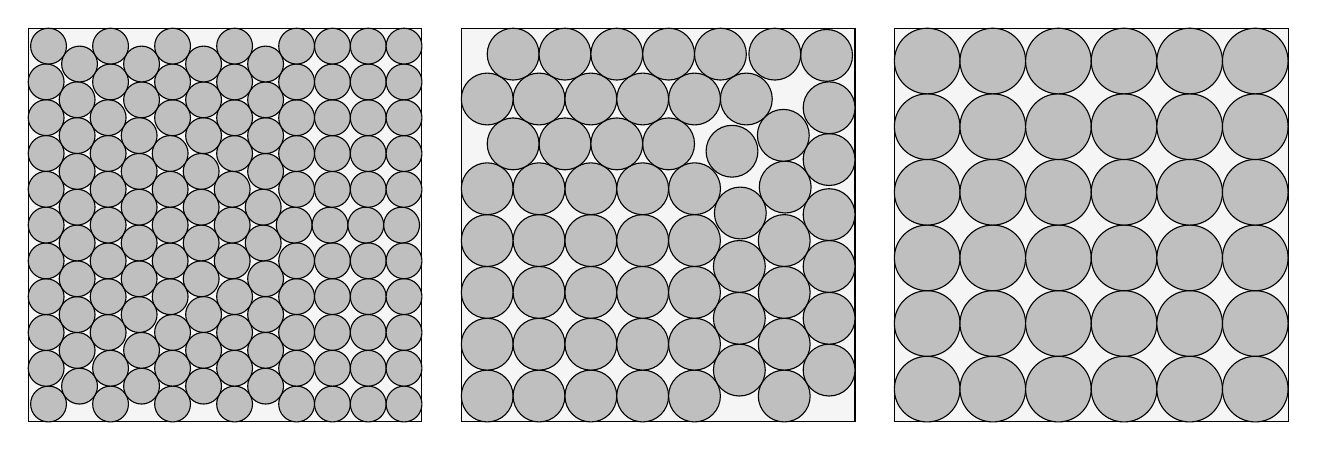
\begin{tikzpicture}[scale=5]
 	\begin{scope}[]
 	\fill[lightgray!15,draw=black] (0,0) rectangle (1,1);
 	\fill[lightgray,draw=black] (0.051591,0.0454733)circle(0.0454732);
 	\fill[lightgray,draw=black] (0.209115,0.0454733)circle(0.0454732);
 	\fill[lightgray,draw=black] (0.366639,0.0454733)circle(0.0454732);
 	\fill[lightgray,draw=black] (0.524163,0.0454733)circle(0.0454732);
 	\fill[lightgray,draw=black] (0.681687,0.0454733)circle(0.0454732);
 	\fill[lightgray,draw=black] (0.772634,0.0454733)circle(0.0454732);
 	\fill[lightgray,draw=black] (0.86358,0.0454733)circle(0.0454732);
 	\fill[lightgray,draw=black] (0.954527,0.0454733)circle(0.0454732);
 	\fill[lightgray,draw=black] (0.130353,0.0909465)circle(0.0454732);
 	\fill[lightgray,draw=black] (0.287877,0.0909465)circle(0.0454732);
 	\fill[lightgray,draw=black] (0.445401,0.0909465)circle(0.0454732);
 	\fill[lightgray,draw=black] (0.602925,0.0909465)circle(0.0454732);
 	\fill[lightgray,draw=black] (0.0454733,0.136214)circle(0.0454732);
 	\fill[lightgray,draw=black] (0.209115,0.13642)circle(0.0454732);
 	\fill[lightgray,draw=black] (0.366639,0.13642)circle(0.0454732);
 	\fill[lightgray,draw=black] (0.524163,0.13642)circle(0.0454732);
 	\fill[lightgray,draw=black] (0.681687,0.13642)circle(0.0454732);
 	\fill[lightgray,draw=black] (0.772634,0.13642)circle(0.0454732);
 	\fill[lightgray,draw=black] (0.86358,0.13642)circle(0.0454732);
 	\fill[lightgray,draw=black] (0.954527,0.13642)circle(0.0454732);
 	\fill[lightgray,draw=black] (0.124235,0.181687)circle(0.0454732);
 	\fill[lightgray,draw=black] (0.287877,0.181893)circle(0.0454732);
 	\fill[lightgray,draw=black] (0.445401,0.181893)circle(0.0454732);
 	\fill[lightgray,draw=black] (0.602925,0.181893)circle(0.0454732);
 	\fill[lightgray,draw=black] (0.0454733,0.22716)circle(0.0454732);
 	\fill[lightgray,draw=black] (0.202997,0.22716)circle(0.0454732);
 	\fill[lightgray,draw=black] (0.366639,0.227366)circle(0.0454732);
 	\fill[lightgray,draw=black] (0.524163,0.227366)circle(0.0454732);
 	\fill[lightgray,draw=black] (0.681687,0.227366)circle(0.0454732);
 	\fill[lightgray,draw=black] (0.772634,0.227366)circle(0.0454732);
 	\fill[lightgray,draw=black] (0.86358,0.227366)circle(0.0454732);
 	\fill[lightgray,draw=black] (0.954527,0.227366)circle(0.0454732);
 	\fill[lightgray,draw=black] (0.124235,0.272634)circle(0.0454732);
 	\fill[lightgray,draw=black] (0.281759,0.272634)circle(0.0454732);
 	\fill[lightgray,draw=black] (0.445401,0.27284)circle(0.0454732);
 	\fill[lightgray,draw=black] (0.602925,0.27284)circle(0.0454732);
 	\fill[lightgray,draw=black] (0.0454733,0.318107)circle(0.0454732);
 	\fill[lightgray,draw=black] (0.202997,0.318107)circle(0.0454732);
 	\fill[lightgray,draw=black] (0.360521,0.318107)circle(0.0454732);
 	\fill[lightgray,draw=black] (0.524163,0.318313)circle(0.0454732);
 	\fill[lightgray,draw=black] (0.681687,0.318313)circle(0.0454732);
 	\fill[lightgray,draw=black] (0.772634,0.318313)circle(0.0454732);
 	\fill[lightgray,draw=black] (0.86358,0.318313)circle(0.0454732);
 	\fill[lightgray,draw=black] (0.954527,0.318313)circle(0.0454732);
 	\fill[lightgray,draw=black] (0.124235,0.36358)circle(0.0454732);
 	\fill[lightgray,draw=black] (0.281759,0.36358)circle(0.0454732);
 	\fill[lightgray,draw=black] (0.439283,0.36358)circle(0.0454732);
 	\fill[lightgray,draw=black] (0.602925,0.363786)circle(0.0454732);
 	\fill[lightgray,draw=black] (0.0454733,0.409053)circle(0.0454732);
 	\fill[lightgray,draw=black] (0.202997,0.409053)circle(0.0454732);
 	\fill[lightgray,draw=black] (0.360521,0.409053)circle(0.0454732);
 	\fill[lightgray,draw=black] (0.518045,0.409053)circle(0.0454732);
 	\fill[lightgray,draw=black] (0.681687,0.409259)circle(0.0454732);
 	\fill[lightgray,draw=black] (0.772634,0.409259)circle(0.0454732);
 	\fill[lightgray,draw=black] (0.86358,0.409259)circle(0.0454732);
 	\fill[lightgray,draw=black] (0.954527,0.409259)circle(0.0454732);
 	\fill[lightgray,draw=black] (0.124235,0.454527)circle(0.0454732);
 	\fill[lightgray,draw=black] (0.281759,0.454527)circle(0.0454732);
 	\fill[lightgray,draw=black] (0.439283,0.454527)circle(0.0454732);
 	\fill[lightgray,draw=black] (0.596807,0.454527)circle(0.0454732);
 	\fill[lightgray,draw=black] (0.0454733,0.5)circle(0.0454732);
 	\fill[lightgray,draw=black] (0.202997,0.5)circle(0.0454732);
 	\fill[lightgray,draw=black] (0.360521,0.5)circle(0.0454732);
 	\fill[lightgray,draw=black] (0.518045,0.5)circle(0.0454732);
 	\fill[lightgray,draw=black] (0.675569,0.5)circle(0.0454732);
 	\fill[lightgray,draw=black] (0.766516,0.5)circle(0.0454732);
 	\fill[lightgray,draw=black] (0.857462,0.5)circle(0.0454732);
 	\fill[lightgray,draw=black] (0.948409,0.5)circle(0.0454732);
 	\fill[lightgray,draw=black] (0.124235,0.545473)circle(0.0454732);
 	\fill[lightgray,draw=black] (0.281759,0.545473)circle(0.0454732);
 	\fill[lightgray,draw=black] (0.439283,0.545473)circle(0.0454732);
 	\fill[lightgray,draw=black] (0.596807,0.545473)circle(0.0454732);
 	\fill[lightgray,draw=black] (0.681687,0.590741)circle(0.0454732);
 	\fill[lightgray,draw=black] (0.772634,0.590741)circle(0.0454732);
 	\fill[lightgray,draw=black] (0.86358,0.590741)circle(0.0454732);
 	\fill[lightgray,draw=black] (0.954527,0.590741)circle(0.0454732);
 	\fill[lightgray,draw=black] (0.0454733,0.590947)circle(0.0454732);
 	\fill[lightgray,draw=black] (0.202997,0.590947)circle(0.0454732);
 	\fill[lightgray,draw=black] (0.360521,0.590947)circle(0.0454732);
 	\fill[lightgray,draw=black] (0.518045,0.590947)circle(0.0454732);
 	\fill[lightgray,draw=black] (0.602925,0.636214)circle(0.0454732);
 	\fill[lightgray,draw=black] (0.124235,0.63642)circle(0.0454732);
 	\fill[lightgray,draw=black] (0.281759,0.63642)circle(0.0454732);
 	\fill[lightgray,draw=black] (0.439283,0.63642)circle(0.0454732);
 	\fill[lightgray,draw=black] (0.524163,0.681687)circle(0.0454732);
 	\fill[lightgray,draw=black] (0.681687,0.681687)circle(0.0454732);
 	\fill[lightgray,draw=black] (0.772634,0.681687)circle(0.0454732);
 	\fill[lightgray,draw=black] (0.86358,0.681687)circle(0.0454732);
 	\fill[lightgray,draw=black] (0.954527,0.681687)circle(0.0454732);
 	\fill[lightgray,draw=black] (0.0454733,0.681893)circle(0.0454732);
 	\fill[lightgray,draw=black] (0.202997,0.681893)circle(0.0454732);
 	\fill[lightgray,draw=black] (0.360521,0.681893)circle(0.0454732);
 	\fill[lightgray,draw=black] (0.445401,0.72716)circle(0.0454732);
 	\fill[lightgray,draw=black] (0.602925,0.72716)circle(0.0454732);
 	\fill[lightgray,draw=black] (0.124235,0.727366)circle(0.0454732);
 	\fill[lightgray,draw=black] (0.281759,0.727366)circle(0.0454732);
 	\fill[lightgray,draw=black] (0.366639,0.772634)circle(0.0454732);
 	\fill[lightgray,draw=black] (0.524163,0.772634)circle(0.0454732);
 	\fill[lightgray,draw=black] (0.681687,0.772634)circle(0.0454732);
 	\fill[lightgray,draw=black] (0.772634,0.772634)circle(0.0454732);
 	\fill[lightgray,draw=black] (0.86358,0.772634)circle(0.0454732);
 	\fill[lightgray,draw=black] (0.954527,0.772634)circle(0.0454732);
 	\fill[lightgray,draw=black] (0.0454733,0.77284)circle(0.0454732);
 	\fill[lightgray,draw=black] (0.202997,0.77284)circle(0.0454732);
 	\fill[lightgray,draw=black] (0.287877,0.818107)circle(0.0454732);
 	\fill[lightgray,draw=black] (0.445401,0.818107)circle(0.0454732);
 	\fill[lightgray,draw=black] (0.602925,0.818107)circle(0.0454732);
 	\fill[lightgray,draw=black] (0.124235,0.818313)circle(0.0454732);
 	\fill[lightgray,draw=black] (0.209115,0.86358)circle(0.0454732);
 	\fill[lightgray,draw=black] (0.366639,0.86358)circle(0.0454732);
 	\fill[lightgray,draw=black] (0.524163,0.86358)circle(0.0454732);
 	\fill[lightgray,draw=black] (0.681687,0.86358)circle(0.0454732);
 	\fill[lightgray,draw=black] (0.772634,0.86358)circle(0.0454732);
 	\fill[lightgray,draw=black] (0.86358,0.86358)circle(0.0454732);
 	\fill[lightgray,draw=black] (0.954527,0.86358)circle(0.0454732);
 	\fill[lightgray,draw=black] (0.0454733,0.863786)circle(0.0454732);
 	\fill[lightgray,draw=black] (0.130353,0.909053)circle(0.0454732);
 	\fill[lightgray,draw=black] (0.287877,0.909053)circle(0.0454732);
 	\fill[lightgray,draw=black] (0.445401,0.909053)circle(0.0454732);
 	\fill[lightgray,draw=black] (0.602925,0.909053)circle(0.0454732);
 	\fill[lightgray,draw=black] (0.051591,0.954527)circle(0.0454732);
 	\fill[lightgray,draw=black] (0.209115,0.954527)circle(0.0454732);
 	\fill[lightgray,draw=black] (0.366639,0.954527)circle(0.0454732);
 	\fill[lightgray,draw=black] (0.524163,0.954527)circle(0.0454732);
 	\fill[lightgray,draw=black] (0.681687,0.954527)circle(0.0454732);
 	\fill[lightgray,draw=black] (0.772634,0.954527)circle(0.0454732);
 	\fill[lightgray,draw=black] (0.86358,0.954527)circle(0.0454732);
 	\fill[lightgray,draw=black] (0.954527,0.954527)circle(0.0454732);
 	\end{scope}[]
 	\begin{scope}[shift={(1.1,0)}]
 	\fill[lightgray!15,draw=black] (0,0) rectangle (1,1);
 	\fill[lightgray,draw=black] (0.0658075,0.0658075)circle(0.0658074);
 	\fill[lightgray,draw=black] (0.197422,0.0658075)circle(0.0658074);
 	\fill[lightgray,draw=black] (0.329037,0.0658075)circle(0.0658074);
 	\fill[lightgray,draw=black] (0.460652,0.0658075)circle(0.0658074);
 	\fill[lightgray,draw=black] (0.592267,0.0658075)circle(0.0658074);
 	\fill[lightgray,draw=black] (0.820231,0.0658075)circle(0.0658074);
 	\fill[lightgray,draw=black] (0.706249,0.131615)circle(0.0658074);
 	\fill[lightgray,draw=black] (0.934193,0.131651)circle(0.0658074);
 	\fill[lightgray,draw=black] (0.0658075,0.197422)circle(0.0658074);
 	\fill[lightgray,draw=black] (0.197422,0.197422)circle(0.0658074);
 	\fill[lightgray,draw=black] (0.329037,0.197422)circle(0.0658074);
 	\fill[lightgray,draw=black] (0.460652,0.197422)circle(0.0658074);
 	\fill[lightgray,draw=black] (0.592267,0.197422)circle(0.0658074);
 	\fill[lightgray,draw=black] (0.820211,0.197458)circle(0.0658074);
 	\fill[lightgray,draw=black] (0.706229,0.263266)circle(0.0658074);
 	\fill[lightgray,draw=black] (0.934193,0.263266)circle(0.0658074);
 	\fill[lightgray,draw=black] (0.0658075,0.329037)circle(0.0658074);
 	\fill[lightgray,draw=black] (0.197422,0.329037)circle(0.0658074);
 	\fill[lightgray,draw=black] (0.329037,0.329037)circle(0.0658074);
 	\fill[lightgray,draw=black] (0.460652,0.329037)circle(0.0658074);
 	\fill[lightgray,draw=black] (0.820211,0.329073)circle(0.0658074);
 	\fill[lightgray,draw=black] (0.592267,0.329109)circle(0.0658074);
 	\fill[lightgray,draw=black] (0.934193,0.394881)circle(0.0658074);
 	\fill[lightgray,draw=black] (0.706249,0.394917)circle(0.0658074);
 	\fill[lightgray,draw=black] (0.0658075,0.460652)circle(0.0658074);
 	\fill[lightgray,draw=black] (0.197422,0.460652)circle(0.0658074);
 	\fill[lightgray,draw=black] (0.329037,0.460652)circle(0.0658074);
 	\fill[lightgray,draw=black] (0.460652,0.460652)circle(0.0658074);
 	\fill[lightgray,draw=black] (0.592267,0.460724)circle(0.0658074);
 	\fill[lightgray,draw=black] (0.820231,0.460724)circle(0.0658074);
 	\fill[lightgray,draw=black] (0.934193,0.526568)circle(0.0658074);
 	\fill[lightgray,draw=black] (0.708711,0.530623)circle(0.0658074);
 	\fill[lightgray,draw=black] (0.329109,0.592267)circle(0.0658074);
 	\fill[lightgray,draw=black] (0.460724,0.592267)circle(0.0658074);
 	\fill[lightgray,draw=black] (0.0658075,0.592267)circle(0.0658074);
 	\fill[lightgray,draw=black] (0.197422,0.592267)circle(0.0658074);
 	\fill[lightgray,draw=black] (0.592463,0.592339)circle(0.0658074);
 	\fill[lightgray,draw=black] (0.822673,0.596466)circle(0.0658074);
 	\fill[lightgray,draw=black] (0.934193,0.666365)circle(0.0658074);
 	\fill[lightgray,draw=black] (0.687571,0.687571)circle(0.0658074);
 	\fill[lightgray,draw=black] (0.263266,0.706229)circle(0.0658074);
 	\fill[lightgray,draw=black] (0.394917,0.706249)circle(0.0658074);
 	\fill[lightgray,draw=black] (0.526532,0.706249)circle(0.0658074);
 	\fill[lightgray,draw=black] (0.131615,0.706249)circle(0.0658074);
 	\fill[lightgray,draw=black] (0.817898,0.727995)circle(0.0658074);
 	\fill[lightgray,draw=black] (0.934192,0.79798)circle(0.0658074);
 	\fill[lightgray,draw=black] (0.197458,0.820211)circle(0.0658074);
 	\fill[lightgray,draw=black] (0.329073,0.820211)circle(0.0658074);
 	\fill[lightgray,draw=black] (0.592375,0.820211)circle(0.0658074);
 	\fill[lightgray,draw=black] (0.72399,0.820211)circle(0.0658074);
 	\fill[lightgray,draw=black] (0.460724,0.820231)circle(0.0658074);
 	\fill[lightgray,draw=black] (0.0658075,0.820231)circle(0.0658074);
 	\fill[lightgray,draw=black] (0.927873,0.930974)circle(0.0658074);
 	\fill[lightgray,draw=black] (0.796298,0.934192)circle(0.0658074);
 	\fill[lightgray,draw=black] (0.131651,0.934193)circle(0.0658074);
 	\fill[lightgray,draw=black] (0.263266,0.934193)circle(0.0658074);
 	\fill[lightgray,draw=black] (0.394881,0.934193)circle(0.0658074);
 	\fill[lightgray,draw=black] (0.526568,0.934193)circle(0.0658074);
 	\fill[lightgray,draw=black] (0.658183,0.934193)circle(0.0658074);
 	\end{scope}[]
 	\begin{scope}[shift={(2.2,0)}]
 	\fill[lightgray!15,draw=black] (0,0) rectangle (1,1);
 	\fill[lightgray,draw=black] (0.0833333,0.0833333)circle(0.0833333333);
 	\fill[lightgray,draw=black] (0.25,0.0833333)circle(0.0833333333);
 	\fill[lightgray,draw=black] (0.416667,0.0833333)circle(0.0833333333);
 	\fill[lightgray,draw=black] (0.583333,0.0833333)circle(0.0833333333);
 	\fill[lightgray,draw=black] (0.75,0.0833333)circle(0.0833333333);
 	\fill[lightgray,draw=black] (0.916667,0.0833333)circle(0.0833333333);
 	\fill[lightgray,draw=black] (0.0833333,0.25)circle(0.0833333333);
 	\fill[lightgray,draw=black] (0.25,0.25)circle(0.0833333333);
 	\fill[lightgray,draw=black] (0.416667,0.25)circle(0.0833333333);
 	\fill[lightgray,draw=black] (0.583333,0.25)circle(0.0833333333);
 	\fill[lightgray,draw=black] (0.75,0.25)circle(0.0833333333);
 	\fill[lightgray,draw=black] (0.916667,0.25)circle(0.0833333333);
 	\fill[lightgray,draw=black] (0.0833333,0.416667)circle(0.0833333333);
 	\fill[lightgray,draw=black] (0.25,0.416667)circle(0.0833333333);
 	\fill[lightgray,draw=black] (0.416667,0.416667)circle(0.0833333333);
 	\fill[lightgray,draw=black] (0.583333,0.416667)circle(0.0833333333);
 	\fill[lightgray,draw=black] (0.75,0.416667)circle(0.0833333333);
 	\fill[lightgray,draw=black] (0.916667,0.416667)circle(0.0833333333);
 	\fill[lightgray,draw=black] (0.0833333,0.583333)circle(0.0833333333);
 	\fill[lightgray,draw=black] (0.25,0.583333)circle(0.0833333333);
 	\fill[lightgray,draw=black] (0.416667,0.583333)circle(0.0833333333);
 	\fill[lightgray,draw=black] (0.583333,0.583333)circle(0.0833333333);
 	\fill[lightgray,draw=black] (0.75,0.583333)circle(0.0833333333);
 	\fill[lightgray,draw=black] (0.916667,0.583333)circle(0.0833333333);
 	\fill[lightgray,draw=black] (0.0833333,0.75)circle(0.0833333333);
 	\fill[lightgray,draw=black] (0.25,0.75)circle(0.0833333333);
 	\fill[lightgray,draw=black] (0.416667,0.75)circle(0.0833333333);
 	\fill[lightgray,draw=black] (0.583333,0.75)circle(0.0833333333);
 	\fill[lightgray,draw=black] (0.75,0.75)circle(0.0833333333);
 	\fill[lightgray,draw=black] (0.916667,0.75)circle(0.0833333333);
 	\fill[lightgray,draw=black] (0.0833333,0.916667)circle(0.0833333333);
 	\fill[lightgray,draw=black] (0.25,0.916667)circle(0.0833333333);
 	\fill[lightgray,draw=black] (0.416667,0.916667)circle(0.0833333333);
 	\fill[lightgray,draw=black] (0.583333,0.916667)circle(0.0833333333);
 	\fill[lightgray,draw=black] (0.75,0.916667)circle(0.0833333333);
 	\fill[lightgray,draw=black] (0.916667,0.916667)circle(0.0833333333);
 	
 	\end{scope}[]
 	\end{tikzpicture}
 	\caption{Most efficient distributions for circle packing for $d=0.1$, $d=0.15$,$d=0.2$.}
 	\label{fig:packing} 
 \end{figure}


With the exception of the latter, these values are yet to be proven to be optimal. However, the optimal values are not expected to be very different, as the remaining area is very limited. The
